% 图 57.2 —— 由 `checks/emit_hand.py` 自动拼出（probe 精测 + prims2 图元分解）
%%
% ⚠ 这是**稿子不是成品**：跑 `checks/checkhand.py 57.2` 看指标 + 看叠合图。
%%
%% ⚠ 待核：
%   · 本图 probe 报出阴影族 1 个 —— **本脚本不生成阴影**（要照原书手写）；prims2 的 strokes 里可能含阴影线，核对时留意别画重
%   · 可疑字形 1 项（空心圈 ⊙ 常被认成字母 o）—— 见文件末
%%
\documentclass[12pt]{standalone}
\usepackage{fontspec}
\setsansfont{Arial}
\newfontfamily\mfallback{DejaVu Sans}
\usepackage{tikz}
\begin{document}
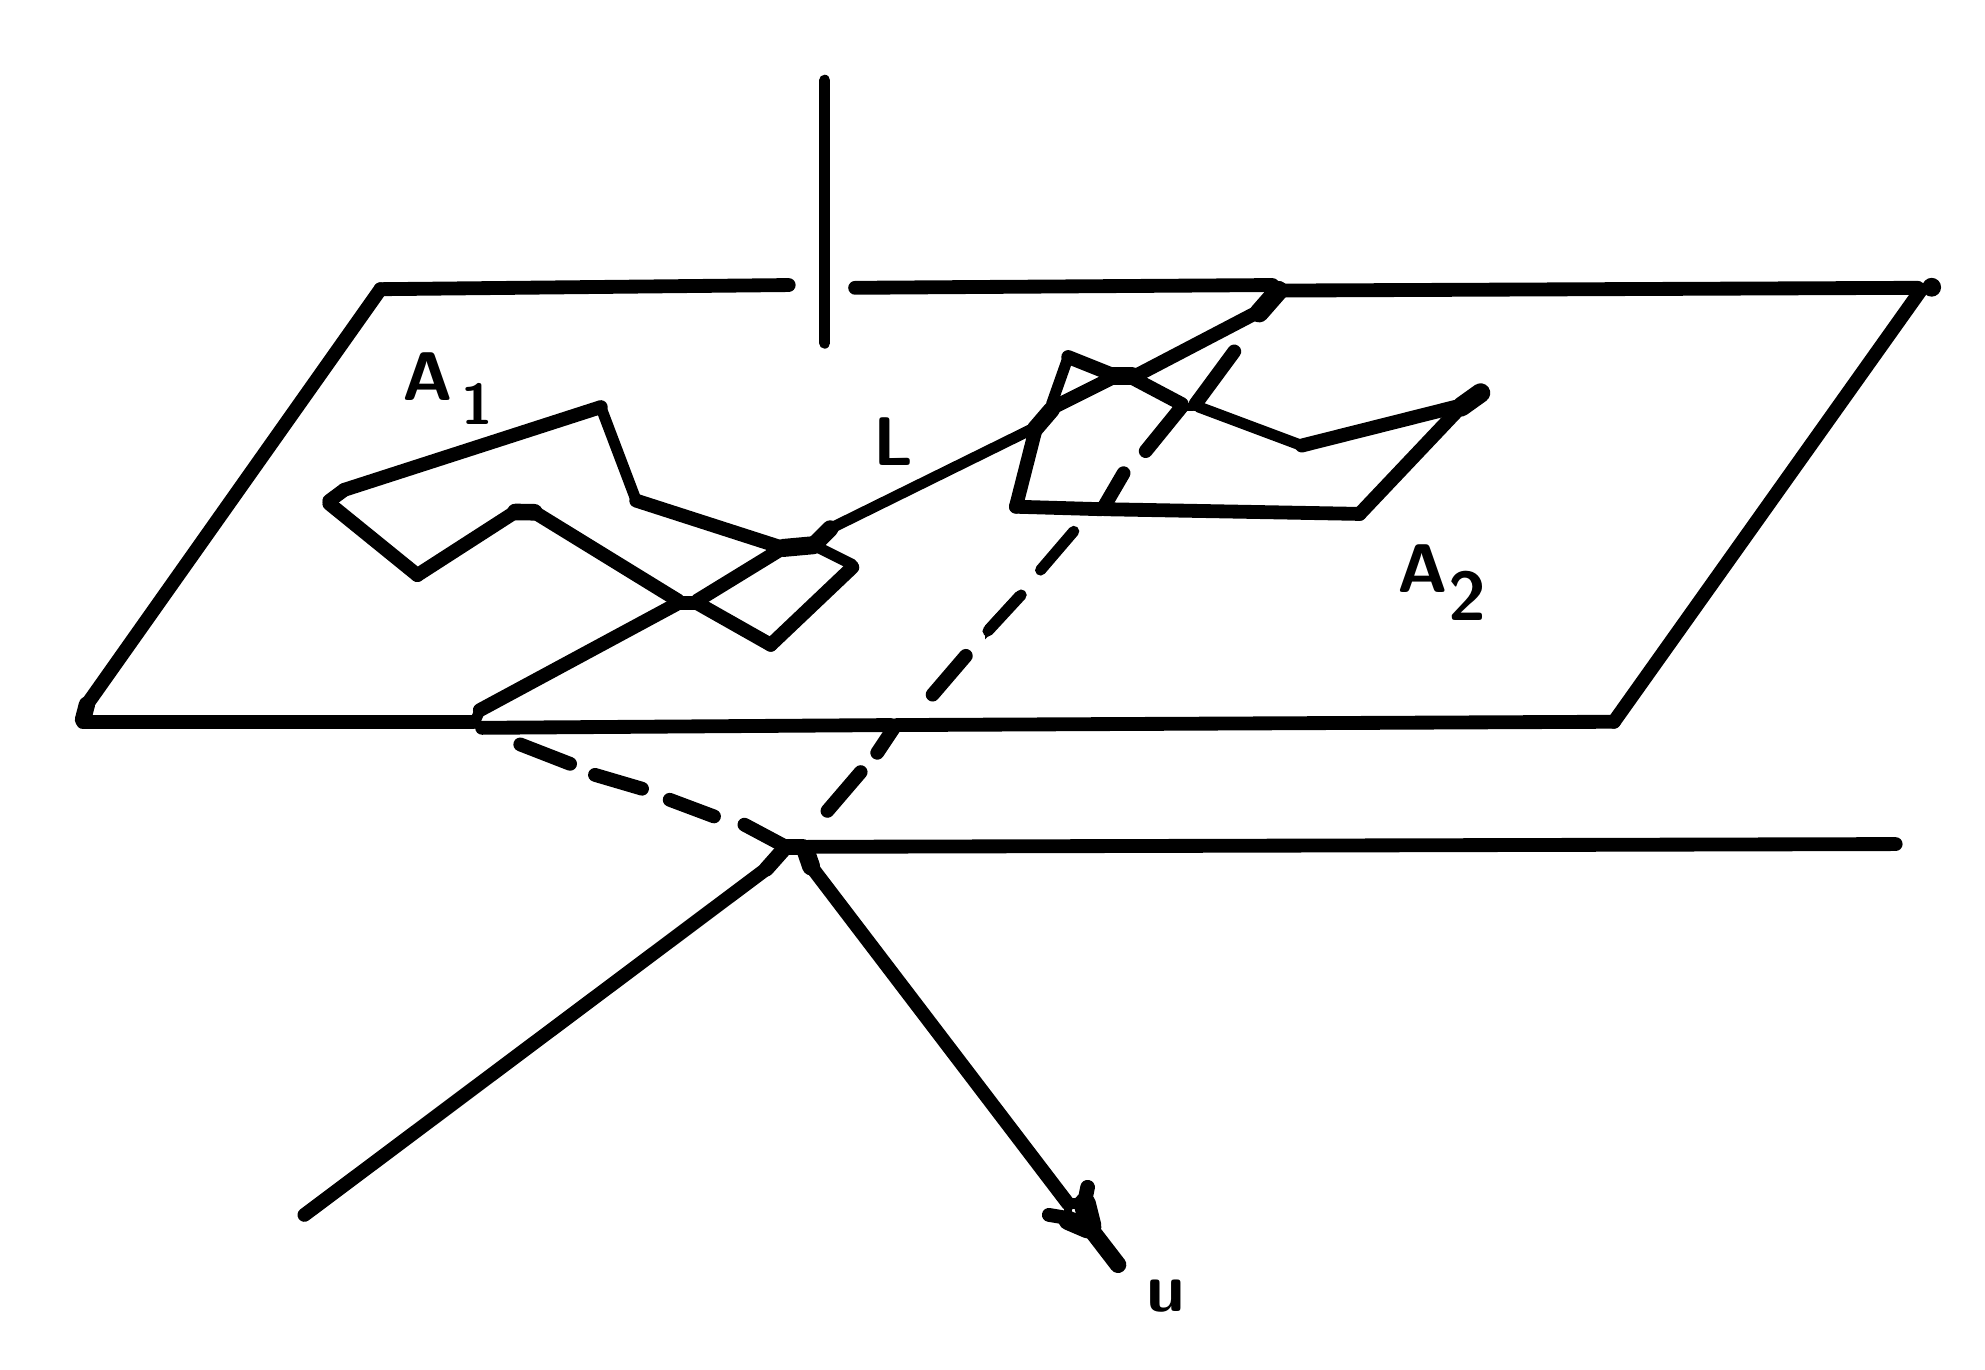
\begin{tikzpicture}[x=1pt, y=-1pt, line width=4.0pt, line cap=round, line join=round]

  %% ════ 填充区（prims2 的 fills）════
  \fill (357.0,204.0) -- (346.0,216.0) -- (346.0,221.0) -- (361.0,205.0) -- cycle;
  \fill (340.0,225.0) -- (337.0,226.0) -- (325.0,240.0) -- (326.0,243.0) -- (328.0,243.0) -- (341.0,227.0) -- cycle;

  %% ════ 直线段（prims2 的 strokes）════
  \draw[line width=4.0pt] (377.0,425.0) -- (381.0,425.0);
  \draw[line width=5.0pt] (100.0,429.0) -- (266.9,304.0);
  \draw[line width=5.5pt] (266.9,304.0) -- (274.0,296.0);
  \draw[line width=7.0pt] (445.0,103.0) -- (452.0,95.0);
  \draw[line width=3.0pt] (376.0,426.0) -- (376.0,429.0);
  \draw[line width=5.0pt] (307.0,262.0) -- (313.0,253.0);
  \draw[line width=5.0pt] (314.0,252.0) -- (573.2,250.8);
  \draw[line width=5.0pt] (573.2,250.8) -- (684.0,95.0);
  \draw[line width=5.0pt] (235.0,208.0) -- (163.4,246.6);
  \draw[line width=3.9pt] (163.4,246.6) -- (162.0,250.0);
  \draw[line width=5.0pt] (109.0,171.0) -- (114.4,167.0);
  \draw[line width=5.0pt] (114.4,167.0) -- (207.1,137.1);
  \draw[line width=4.0pt] (207.1,137.1) -- (219.9,170.9);
  \draw[line width=5.0pt] (219.9,170.9) -- (273.0,188.0);
  \draw[line width=3.0pt] (452.0,95.0) -- (449.8,93.0);
  \draw[line width=5.0pt] (449.8,93.0) -- (299.0,94.0);
  \draw[line width=5.0pt] (452.0,95.0) -- (683.0,94.0);
  \draw[line width=6.0pt] (364.0,145.0) -- (370.0,138.0);
  \draw[line width=5.0pt] (375.0,430.0) -- (369.0,429.0);
  \draw[line width=4.0pt] (370.0,136.0) -- (376.0,119.0);
  \draw[line width=5.0pt] (376.0,119.0) -- (391.0,125.0);
  \draw[line width=5.0pt] (389.0,173.0) -- (396.0,161.0);
  \draw[line width=7.0pt] (376.0,431.0) -- (383.0,434.0);
  \draw[line width=6.0pt] (384.0,434.0) -- (394.0,447.0);
  \draw[line width=5.0pt] (178.0,259.0) -- (196.0,266.0);
  \draw[line width=4.0pt] (366.0,196.0) -- (378.0,182.0);
  \draw[line width=6.5pt] (273.0,188.0) -- (284.0,187.0);
  \draw[line width=5.0pt] (273.0,188.0) -- (242.0,207.0);
  \draw[line width=5.3pt] (382.0,424.0) -- (383.0,419.0);
  \draw[line width=5.0pt] (404.0,153.0) -- (417.0,137.0);
  \draw[line width=5.0pt] (371.0,137.0) -- (391.0,127.0);
  \draw[line width=5.0pt] (222.0,275.0) -- (205.0,270.0);
  \draw[line width=5.0pt] (327.0,241.0) -- (339.0,227.0);
  \draw[line width=5.0pt] (259.0,288.0) -- (274.0,296.0);
  \draw[line width=5.0pt] (400.0,126.0) -- (444.0,103.0);
  \draw[line width=6.0pt] (274.0,296.0) -- (280.0,296.0);
  \draw[line width=5.0pt] (388.0,174.0) -- (357.1,173.1);
  \draw[line width=5.0pt] (357.1,173.1) -- (364.0,146.0);
  \draw[line width=5.0pt] (675.0,295.0) -- (282.0,296.0);
  \draw[line width=5.0pt] (422.0,136.0) -- (436.0,117.0);
  \draw[line width=3.0pt] (421.0,137.0) -- (418.0,137.0);
  \draw[line width=3.0pt] (162.0,251.0) -- (164.2,253.0);
  \draw[line width=5.0pt] (164.2,253.0) -- (312.0,252.0);
  \draw[line width=7.0pt] (525.0,132.0) -- (518.0,137.0);
  \draw[line width=5.0pt] (248.0,285.0) -- (232.0,279.0);
  \draw[line width=4.0pt] (363.0,145.0) -- (290.0,181.0);
  \draw[line width=6.0pt] (290.0,181.0) -- (284.0,187.0);
  \draw[line width=4.0pt] (423.0,137.0) -- (460.4,151.0);
  \draw[line width=5.0pt] (460.4,151.0) -- (516.0,137.0);
  \draw[line width=4.0pt] (359.0,205.0) -- (347.0,218.0);
  \draw[line width=5.0pt] (417.0,136.0) -- (400.0,127.0);
  \draw[line width=5.0pt] (20.0,251.0) -- (161.0,251.0);
  \draw[line width=5.0pt] (275.0,93.0) -- (127.5,94.5);
  \draw[line width=5.0pt] (127.5,94.5) -- (21.4,244.6);
  \draw[line width=5.9pt] (21.4,244.6) -- (20.0,250.0);
  \draw[line width=5.0pt] (241.0,208.0) -- (236.0,208.0);
  \draw[line width=5.0pt] (376.0,425.0) -- (283.1,303.1);
  \draw[line width=6.5pt] (283.1,303.1) -- (281.0,297.0);
  \draw[line width=5.0pt] (298.0,195.0) -- (268.5,223.0);
  \draw[line width=5.0pt] (268.5,223.0) -- (242.0,208.0);
  \draw[line width=4.0pt] (288.0,114.0) -- (288.0,19.0);
  \draw[line width=5.0pt] (235.0,207.0) -- (183.1,175.1);
  \draw[line width=6.0pt] (183.1,175.1) -- (176.2,175.0);
  \draw[line width=5.0pt] (176.2,175.0) -- (140.8,197.8);
  \draw[line width=5.0pt] (140.8,197.8) -- (109.0,172.0);
  \draw[line width=6.5pt] (399.0,126.0) -- (392.0,126.0);
  \draw[line width=5.0pt] (301.0,269.0) -- (289.0,283.0);
  \draw[line width=5.0pt] (389.0,174.0) -- (481.3,175.7);
  \draw[line width=5.0pt] (481.3,175.7) -- (517.0,138.0);
  \draw[line width=8.0pt] (384.0,433.0) -- (382.0,425.0);
  \draw[line width=4.0pt] (284.0,187.0) -- (298.0,194.0);

  %% ════ 实心点 ════
  \fill (688.0,93.8) circle (3.4);

  %% ════ 标签（probe 直接给的 \node 行）════
  %% ⚠ 全部补了 fill=white：文字在最上层，否则与曲线交叉干扰
     \node[anchor=center,inner sep=0pt,fill=white,font=\fontsize{28.1}{35.2}\selectfont] at (144.6,126.0) {\textsf{\textbf{\textit{A}}}};   % box(133,115,18,21)
     \node[anchor=center,inner sep=0pt,fill=white,font=\fontsize{20.6}{25.7}\selectfont] at (162.4,136.3) {\textsf{\textbf{1}}};   % box(157,128,6,16)
     \node[anchor=center,inner sep=0pt,fill=white,font=\fontsize{30.0}{37.6}\selectfont] at (312.8,149.5) {\textsf{\textbf{\textit{L}}}};   % box(304,137,15,23)
     \node[anchor=center,inner sep=0pt,fill=white,font=\fontsize{29.6}{37.0}\selectfont] at (504.2,195.5) {\textsf{\textbf{\textit{A}}}};   % box(492,184,19,22)
     \node[anchor=center,inner sep=0pt,fill=white,font=\fontsize{22.9}{28.7}\selectfont] at (520.1,205.4) {\textsf{\textbf{2}}};   % box(514,197,11,16)
     \node[anchor=center,inner sep=0pt,fill=white,font=\fontsize{31.4}{39.2}\selectfont] at (411.1,458.3) {\textsf{\textbf{\textit{u}}}};   % box(401,448,17,17)

  % 钉死画布：否则超出的图元/控制点会把页面撑大，1:1 回比就失准
  \pgfresetboundingbox
  \path[use as bounding box] (0,0) rectangle (697,475);
\end{tikzpicture}
\end{document}

% ⚠ 待核清单（probe 拿不准，人眼过一遍）：
%   · 未识别/跳过：⑤ 跳过/未识别的字形
